\documentclass{article}
\usepackage[utf8]{inputenc}
\usepackage{subfiles}
\usepackage{amsmath}
\usepackage{amsthm}
\usepackage{amssymb}
\usepackage{graphicx}
\usepackage{wrapfig}
\usepackage{float}
\usepackage{fancyhdr}
\usepackage{booktabs}
\usepackage{pst-node}
\usepackage{hyperref}
\usepackage{tikz-cd} 
\usepackage[a4paper, total={6.5in, 9.5in}]{geometry}
\setlength{\parindent}{0pt}
\newtheorem{defn}{Definition}[section]
\newtheorem{prop}[defn]{Proposition}
\newtheorem{thm}[defn]{Theorem}
\newtheorem{crl}[defn]{Corollary}
\newtheorem{lemma}[defn]{Lemma}
\newtheorem{ex}[defn]{Example}
\renewcommand\qedsymbol{QED}
\newcommand{\bigzero}{\mbox{\normalfont\Large\bfseries 0}}
\newcommand{\rvline}{\hspace*{-\arraycolsep}\vline\hspace*{-\arraycolsep}}
\usepackage[shortlabels]{enumitem}
\newcommand{\subscript}[2]{$#1 _ #2$}
\usepackage{subfiles}
\usepackage{graphicx,subfig}
\usepackage{pdfpages}
% NEW COMMANDS FOR SHORTCUTS
\newcommand{\bb}[1]{\mathbb{#1}}
\newcommand{\soc}[1]{\overline{\text{soc}}^{#1}}
\newcommand{\res}[1]{\text{res}^{#1}}
\newcommand{\tof}[1]{\xrightarrow[]{#1}}
\newcommand{\im}[1]{\text{im }{#1}}
\newcommand{\LR}[3]{\text{N}^{#1}_{#2, #3}}

\title{\textbf{On the structure of injective tensor $\mathfrak{sp}_\infty$-, $\mathfrak{so}_\infty$- modules}\textbf{ and of injective resolutions of simple tensor } $\mathfrak{sp}_\infty$\textbf{-}, $ \mathfrak{so}_\infty$\textbf{-modules}}
\author{Diana-Maria Harambas \\ \\ Thesis supervisor: Prof. Dr. Ivan Penkov \\}
\date{Spring 2025}

\begin{document}
\maketitle
\begin{center}
    \vspace{3cm}
    \textbf{Abstract}
\end{center}

\subfile{00-abstract.tex}
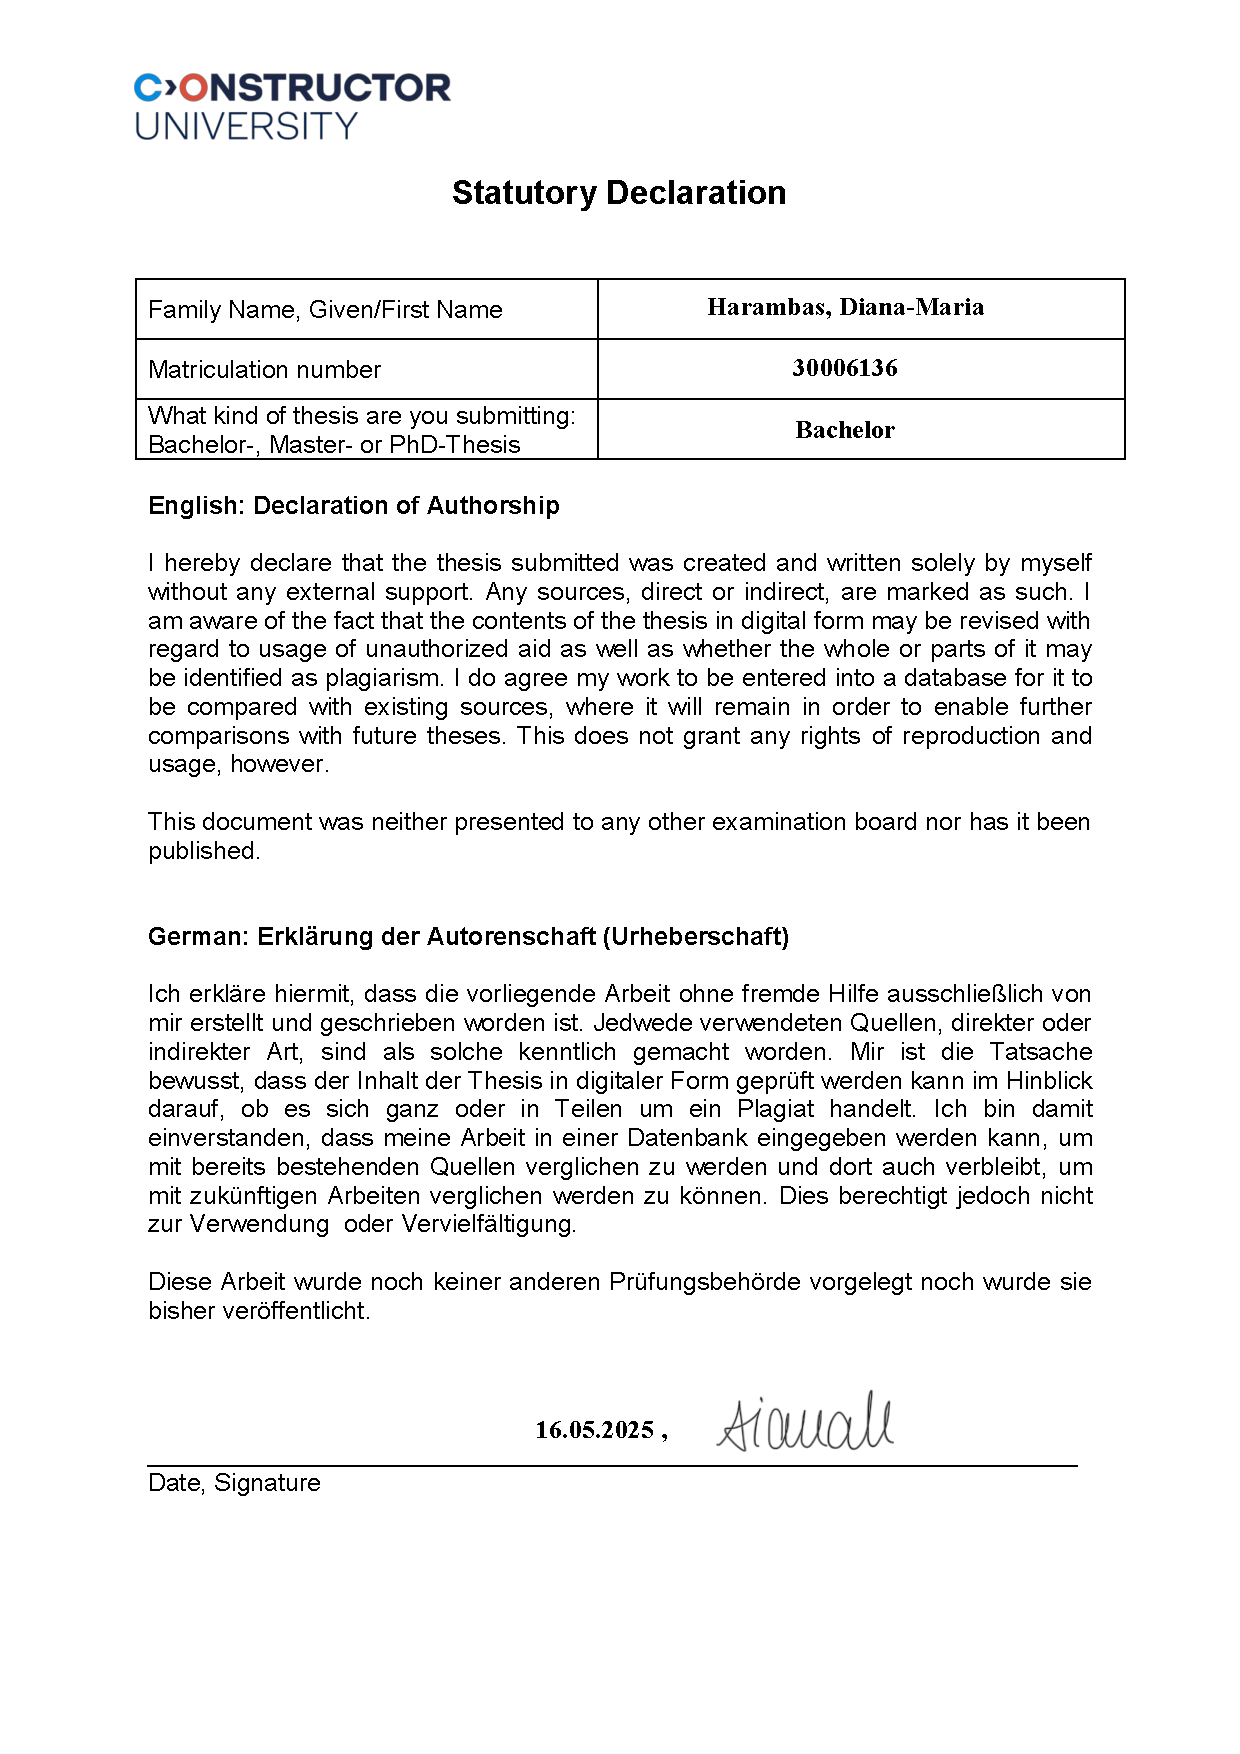
\includepdf[pages={1}]{StatutoryDeclaration.pdf}
\newpage
\setcounter{tocdepth}{2}
\tableofcontents
\newpage


\section{Introduction}
\subfile{01-introduction.tex}

\section{Preliminaries}
\subfile{02-preliminaries.tex}

\section{Length and top layer of socle filtrations of injective tensor $\mathfrak{sp}_\infty$-modules}
\subfile{03-socle-filtrations.tex}

\section{Length and last term of the minimal injective resolutions of simple tensor $\mathfrak{sp}_\infty-$modules}
\subfile{04-resolutions.tex}

\section{The case of tensor $\mathfrak{so}_\infty-$modules}
\subfile{05-so_infty.tex}

\section{Conclusion and outlook}
\subfile{06-conclusion.tex}
\newpage
\section{Appendix}
\subfile{07-appendix.tex}
\newpage
\nocite{*}
\bibliographystyle{alpha}
\bibliography{references}
\end{document}

